\section{Studies of signal and background separation using jet substructure variables}
In this section, we study different jet substructure variables and compare their ability to separate signal from background with different detector sizes and c.m. energy using Mann-Whitney U test and ROC curves.\\

By definition of Mann Whitney U test, if U value is close to 0.5, it means two distributions have similar compositions, and we can not distinguish them very well. On the other hand, if U value of two distributions are close to 0, it means both compositions of both distribution are much different from each other.\\

\subsection{N-subjettiness}
N-subjettiness[\ref{}] is the detection technique of jet substructure that is used to identify boosted hadronically-decaying objects under the high c.m. conditions. We use $\tau$ variable to distinguish the number of subjet in a fatjet to separate signal and background with different detector sizes and c.m. energy.\\

\subsubsection{The technic of N-subjettiness}
The formula and the technique are as following:\\
\begin{equation}\label{eq:Nsub_1}
\tau_{N}=\frac{1}{d_{0}}\sum_{k}p_{T,k} min\{\Delta R_{1,k},\Delta R_{2,k},.....\Delta R_{N,k}\}
\end{equation}
\begin{equation}
d_{0}=\sum_{k}p_{T,k} R_{0}
\end{equation}
k runs over all constituent particles in the given jets (fatjet), $p_{T,k}$ are their transverse momentum, $\Delta R_{J,k}=\sqrt{(\Delta \eta)^{2}+(\Delta \phi)^{2}}$ is the distance between the constituent particles k and the candidate subjet J on the $\eta-\phi$ plane. $R_{0}$ is the characteristic jet radius used in Anti-kt(AK) jet algorithm at starting. $d_{0}$ is the normalization factor.\\
\begin{enumerate}
\item First, Anti-kt(AK) algorithm is used to reconstruct jets
\item Second, after reconstructing the AK4 jets, exclusive $k_{T}$ algorithm[\ref{}] is used in finding the jet axis in a fatjet.
\item Third, start running formula [\ref{eq:Nsub_1}] and loop all constituent particles in a fatjet.
\item Finally, when finishing running all particles, it will give out $\tau_{N}$, where N is positive integer. 
\end{enumerate}

If a fatjet has N subjet(s)[\ref{}], its $\tau_{N}$ is smaller than the $\tau_{N}$ of the fatjet with different number of subjets. For example, if we compare the  $\tau_{2}$ of one-subjet fatjet and two-subjets one, two-subjets fatjet has smaller $\tau_{2}$ than one-subjet one. On the other hand, one-subjet fatjet has smaller $\tau_{1}$ than two-subjets one. In the end, we can use the ratio of  $\tau_{2}$ and  $\tau_{1}$ ( $\tau_{21}$) to distinguish fatjet with one-subjet case and-two subjets case.$\tau_{21}$ is used to discriminate the fatjet shape, and it can be modified with different number of subjet.\\

In our study, we use $\tau_{21}$  and $\tau_{32}$ in distinguishing two-subjets fatjet and three-subjets fatjet from one-subjet fatjet individually. We want to use this two ratio values to distinguish signal from background.\\
\subsubsection{Analysis method}
First, we select the events in mass window by using SD with $\beta=0$ and 75$\%$ signal efficiency. Then, we find the highest ratio bin to be our seed bin. Next, we compare the left and right of ratio bin, and add the higher bin to be our width. Finally,  We can use this width to draw the ROC curves.\\2
\subsubsection{The results and conclusion}
In the figure [\ref{fig:Rawhit_05GeV_tau21_Dis}][\ref{fig:Rawhit_05GeV_tau32_Dis}], they show the histograms of $\tau_{21}$ and $\tau_{32}$ after selecting the events. In all figures, they also include the Mann-Whitney U value in ir the legend.\\

As a result of figure [\ref{fig:Rawhit_05GeV_tau21_ROC}][\ref{fig:Rawhit_05GeV_tau32_ROC}], they perform the ROC curves of $\tau_{21}$ and $\tau_{32}$ with different detector cell sizes and c.m. energy. The smallest detector cell (1$\times$1) doesn't have the best separation power to distinguish signal from background. Some of them have the best separation power with the bigger cell size (5$\times$5 and 20$\times$20).\\

In Figure [\ref{fig:Rawhit_05GeV_total_Mann}](a)(b), they show the summary plots of $\tau_{21}$ and $\tau_{32}$ with the rawhit cut with 0.5GeV using Mann Whitney U test. In $\tau_{21}$, 5TeV has better separation power when detector sizes get smaller. When energy increases, there is no improvement in the smallest detector cell size (1$\times$1). In $\tau_{32}$, the case is similar to  $\tau_{21}$. Even worse, with some c.m. energies, the bigger detector sizes (5$\times$5 and 20$\times$20) have better separation power than the smallest detector sizes (1$\times$1). 
\subsection{Studies of signal and background separation using jet substracture variable: Energy correlation function}
Energy correlation function (ECF) [\ref{}] is another kind of detection technique of jet substructure that is used to distinguish the number of subjets in a fatjet under high c.m. energy conditions. This method only uses the momenta of particles and the angles between them without additional algorithm.\\
\subsubsection{The technic of energy correlation function}
The basic ECF formula is as following:\\
\begin{equation} \label{eq:ECF_Original}
ECF(N,\beta)=\sum_{i_{1}<i_{2}<....<i_{N}\in J} (\prod_{a=1}^{N}E_{ia})(\prod_{b=1}^{N-1}\prod_{c=b+1}^{N} \theta_{i_{b}i_{c}})^{\beta}
\end{equation}

In the formula \ref{eq:ECF_Original}, the sum loop all particles in the jet $J$, $E$ are the energy of particles, and $\theta$ are the angles between the particles.

We apply two approximation. First, because under the high energy limitation $p>>m$, $E\approx p$. Second, we use Radius R between particles naturally, so our ECF formula (\ref{eq:ECF_Original}) can be modified to the formula:\\  
\begin{equation} \label{eq:ECF_Modified}
ECF(N,\beta)=\sum_{i_{1}<i_{2}<....<i_{N}\in J} (\prod_{a=1}^{N}P_{ia})(\prod_{b=1}^{N-1}\prod_{c=b+1}^{N} R_{i_{b}i_{c}})^{\beta}
\end{equation}

From the modified ECF formula (\ref{eq:ECF_Modified}), in order to use the dimensionless observation to determine whether the number of subjets in system, parameter $\tau_{N}$ is defined as:\\
\begin{equation} \label{eq:ECF_ratio}
\tau_{N}^{(\beta)}\equiv\frac{ECF(N+1,\beta)}{ECF(N,\beta)}
\end{equation}

The idea of formula (\ref{eq:ECF_ratio}) is from N-subjetness, because the behavior of it is very similar to N-subjetness as reference [\ref{}]. In general, if the system has N subjets, $ECF(N+1,\beta)$ should be significantly smaller than $ECF(N,\beta)$, so we can use this advantage to distinguish different number of subjets. FInally, because it is suggested to used $\tau_{21}$, $\tau_{32}$ [\ref{}] to distinguish two-subjets fatjet and three-subjets fatjet from one-subjet fatjet, in the ECF, it also defines the ratio of $\tau$ there, and define the energy correlation double ratio that is used in our study:\\
\begin{equation}
C_{N}^{(\beta)}\equiv\frac{\tau_{N}^{(\beta)}}{\tau_{N-1}^{(\beta)}}=\frac{ECF(N-1,\beta)ECF(N+1,\beta)}{ECF(N,\beta)^2}
\end{equation}

We set N=2 and $\beta=1$ ($C_{2}^{1}$) to distinguish two-subjets fatjet from one-subjet fatjet.
\subsubsection{Analysis method}
First, we select the events in mass window by using SD with $\beta=0$ and 75$\%$ signal efficiency. Then, we find the highest ratio bin to be our seed bin. Next, we compare the left and right of ratio bin, and add the higher bin to be our width. Finally,  We can use this width to draw the ROC curves.\\
\subsubsection{The results and conclusion}
In the figure [\ref{fig:Rawhit_05GeV_c2b1_Dis}], they show the histograms of $\tau_{21}$ and $\tau_{32}$ after selecting the events. In all figures, they also include the Mann-Whitney U value in their legend\\

As a result of figure [\ref{fig:Rawhit_05GeV_c2b1_ROC}], they perform the ROC curves of $C_{2}^{1}$ with different detector cell sizes and c.m. energy. The smallest detector cell (1$\times$1) doesn't have the best separation power to distinguish signal from background. In addition, in some cases such like (a), the biggest one (20$\times$20) has the best distinguish power under the same c.m. energy.\\

In Figure [\ref{fig:Rawhit_05GeV_total_Mann}](c), it shows the summary plots with the raw hit cut with 0.5GeV using Mann Whitney U test. For conclusion, all separation power aren't improved by smallest cell size (1$\times$1).\\

%25bins
\begin{figure}
\centering
\begin{center}
   \subfigure[20$\times$20($cm^2$)] {
   \centering
   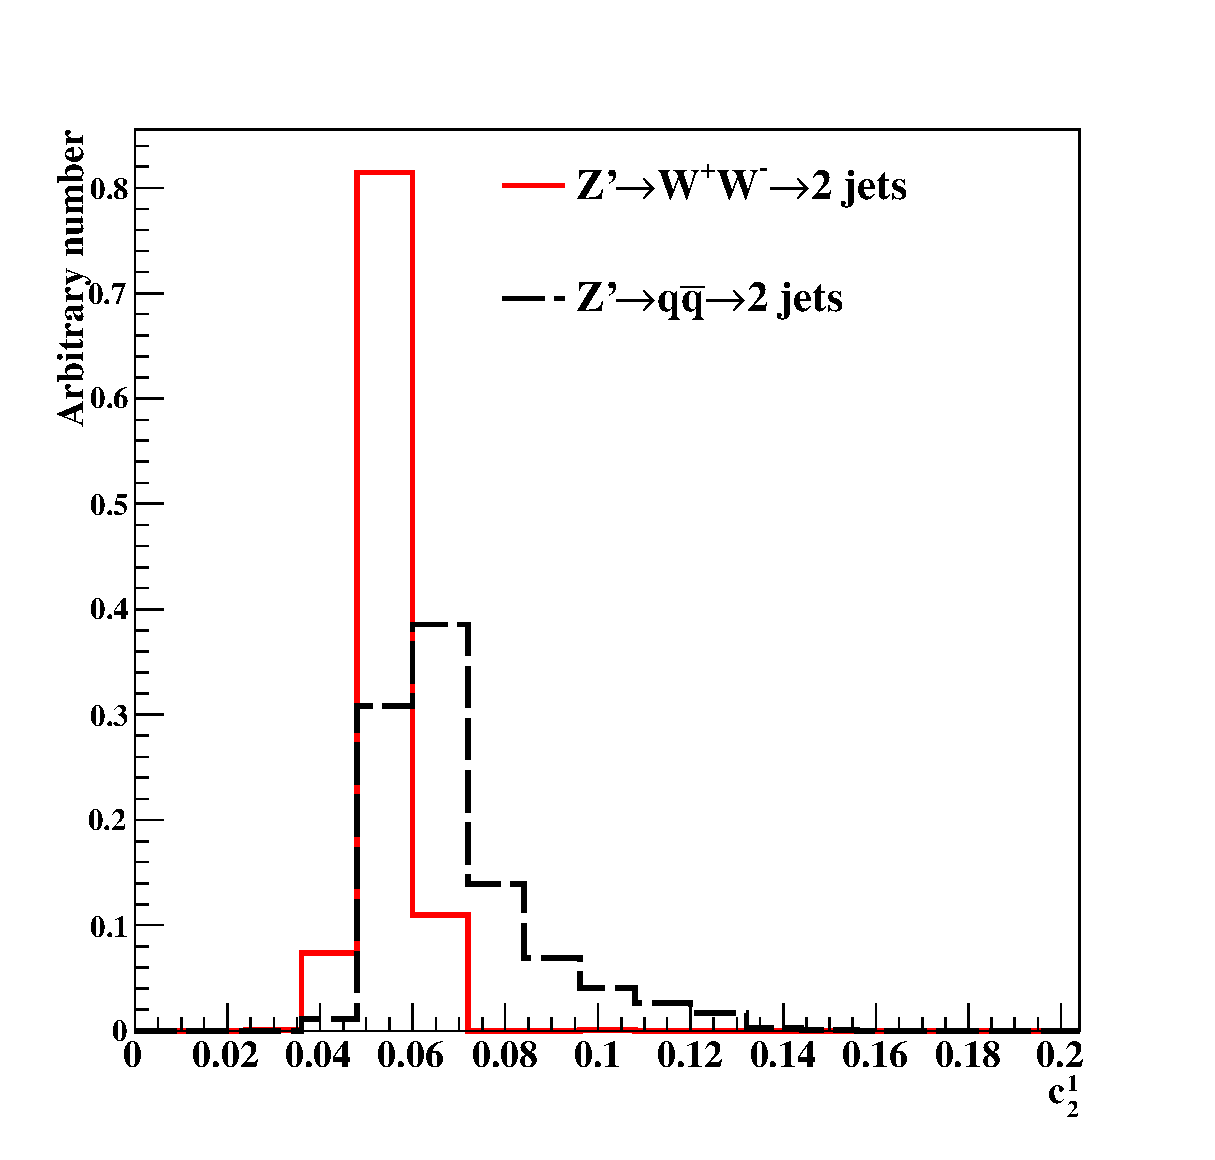
\includegraphics[width=0.3\textwidth]{h_Tau_C/Dis_Rawhit_05GeV_010_c2b1_20tev_04_after_cut_Man_25_no_UOF_new_75pa_for_paper.eps}
   }
   \subfigure[5$\times$5($cm^2$)] {
   \centering
   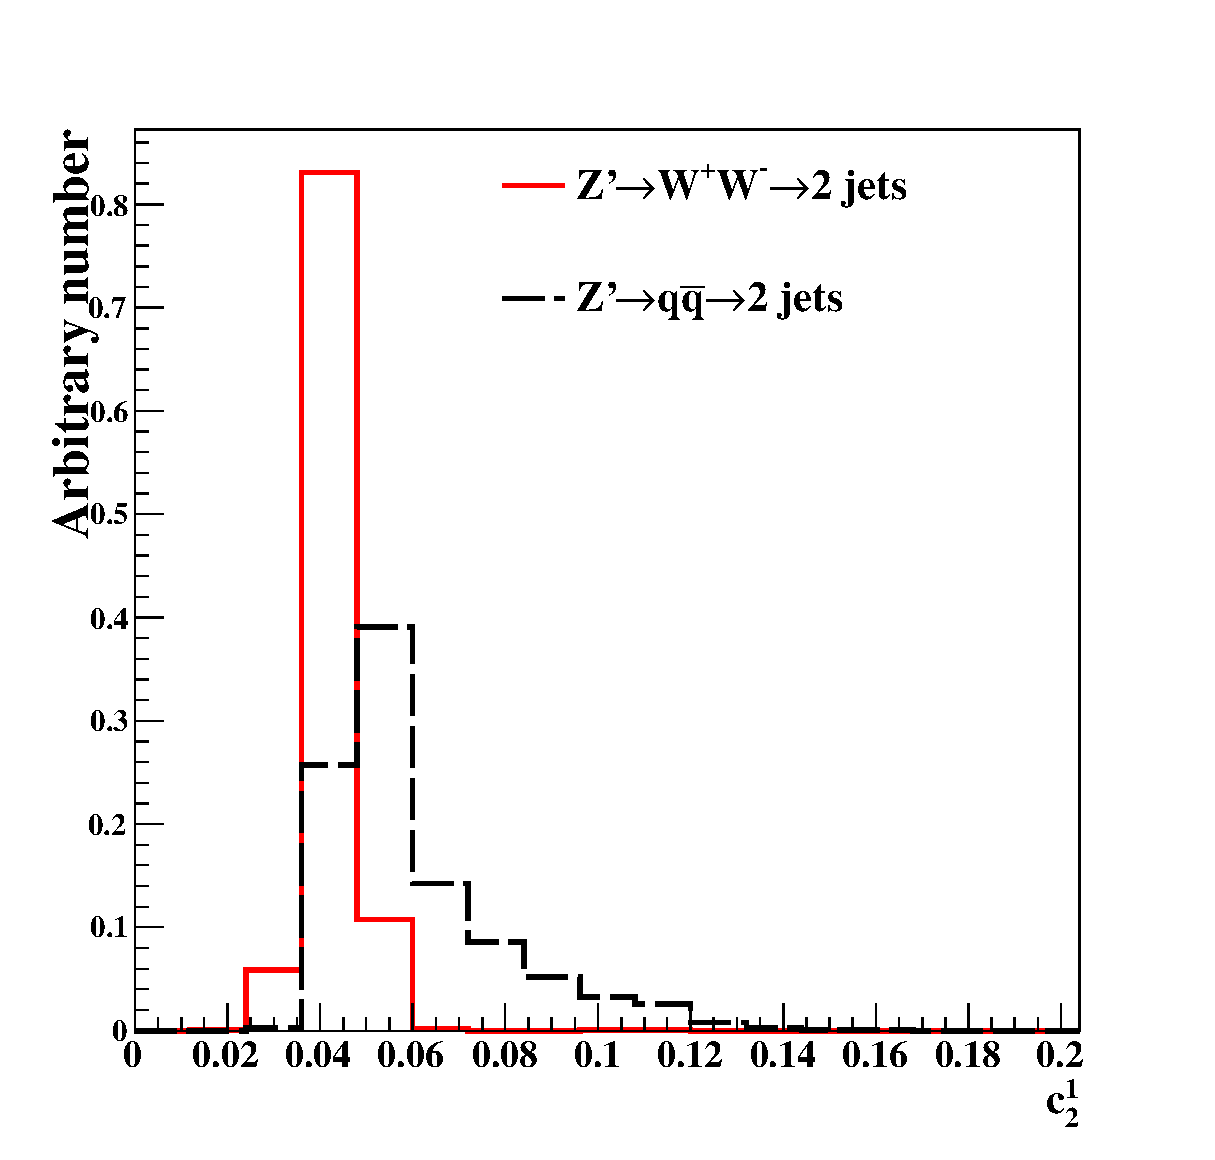
\includegraphics[width=0.3\textwidth]{h_Tau_C/Dis_Rawhit_05GeV_009_c2b1_20tev_04_after_cut_Man_25_no_UOF_new_75pa_for_paper.eps}
   }
   \subfigure[1$\times$1($cm^2$)] {
   \centering
   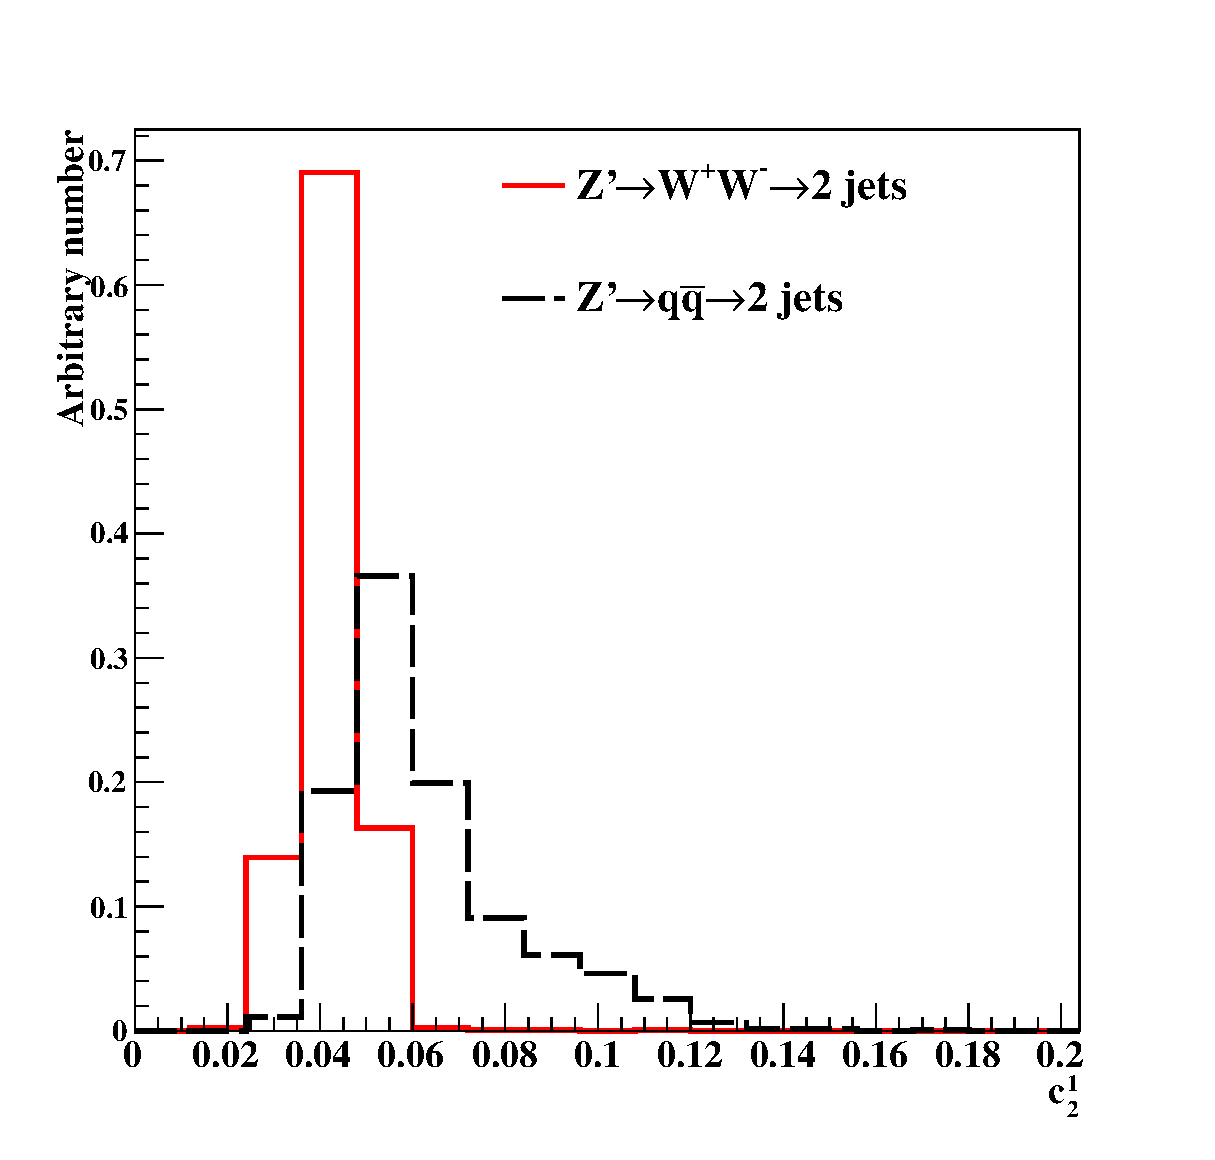
\includegraphics[width=0.3\textwidth]{h_Tau_C/Dis_Rawhit_05GeV_012_c2b1_20tev_04_after_cut_Man_25_no_UOF_new_75pa_for_paper.eps}
   }
\end{center}
\caption{Distributions of Mann-Whitney value U in 20 TeV energy collision for c2b1 in different detector sizes. Cell Size in 20$\times$20, 5$\times$5, and 1$\times$1(cm$\times$cm) are shown here.}
\label{fig:Rawhit_05GeV_c2b1_Dis}
\end{figure}

\begin{figure}
\begin{center}
   \subfigure[Z'(5 TeV)] {
   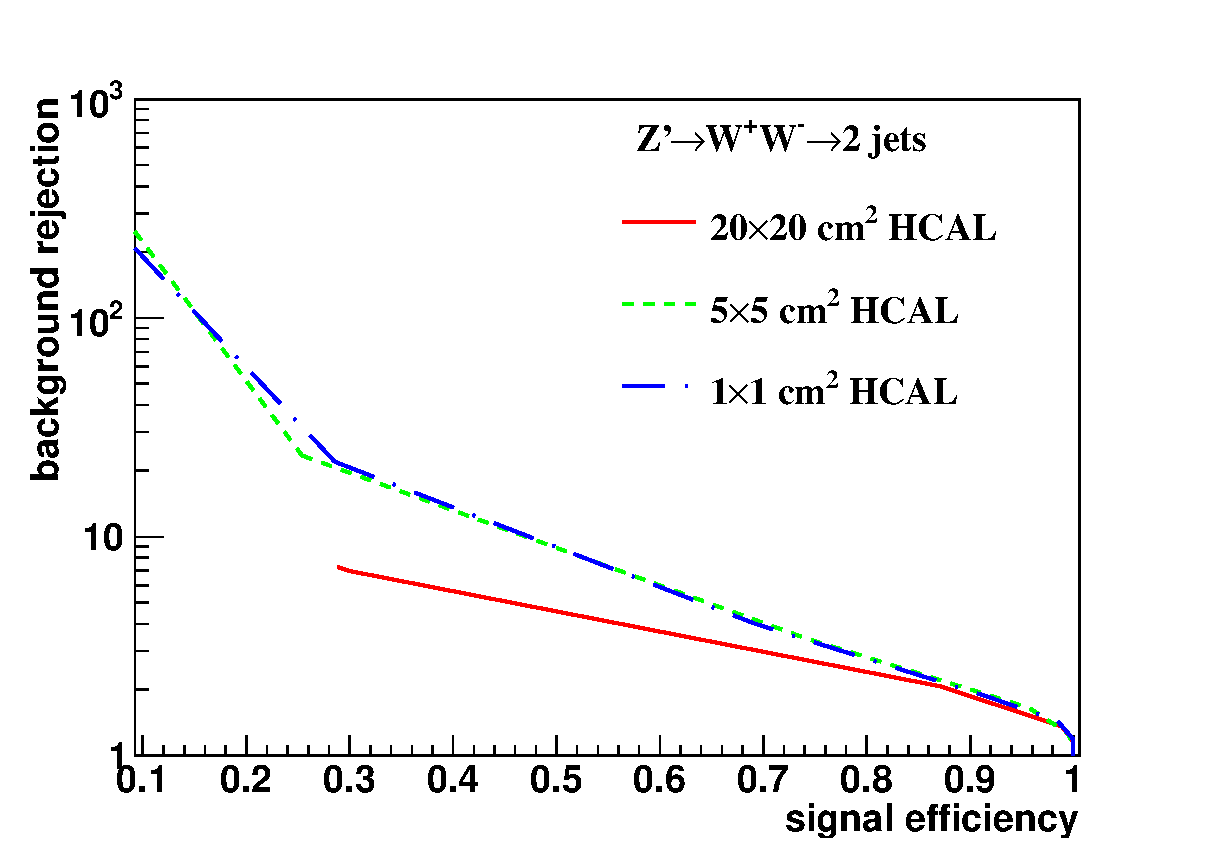
\includegraphics[width=0.43\textwidth]{ROC_Tau_C/Rawhit_05GeV_c2b1_5tev_eff_1_New2_after_cut_25bins_no_UOF_new_75pa.eps}\hfill
   }
   \subfigure[Z'(10 TeV)] {
   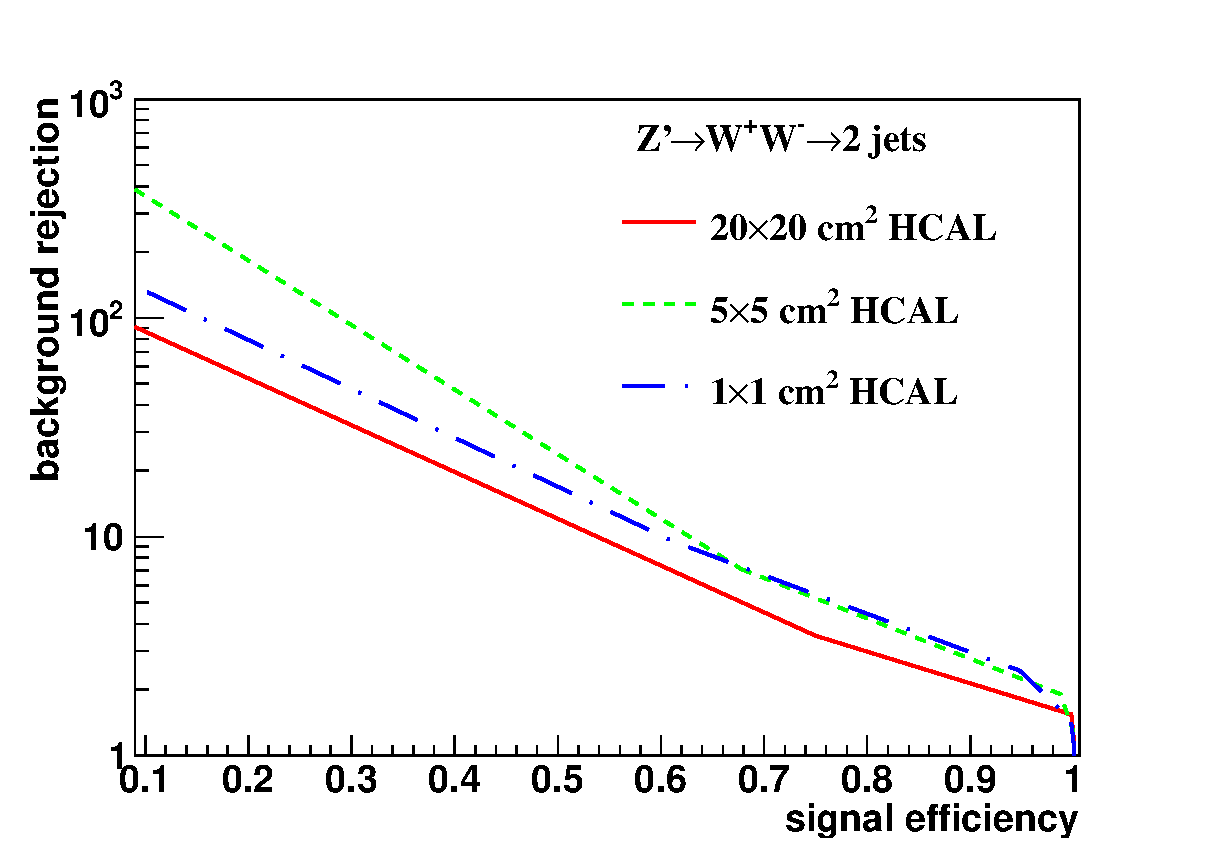
\includegraphics[width=0.43\textwidth]{ROC_Tau_C/Rawhit_05GeV_c2b1_10tev_eff_1_New2_after_cut_25bins_no_UOF_new_75pa.eps}
   }
   \subfigure[Z'(20 TeV)] {
   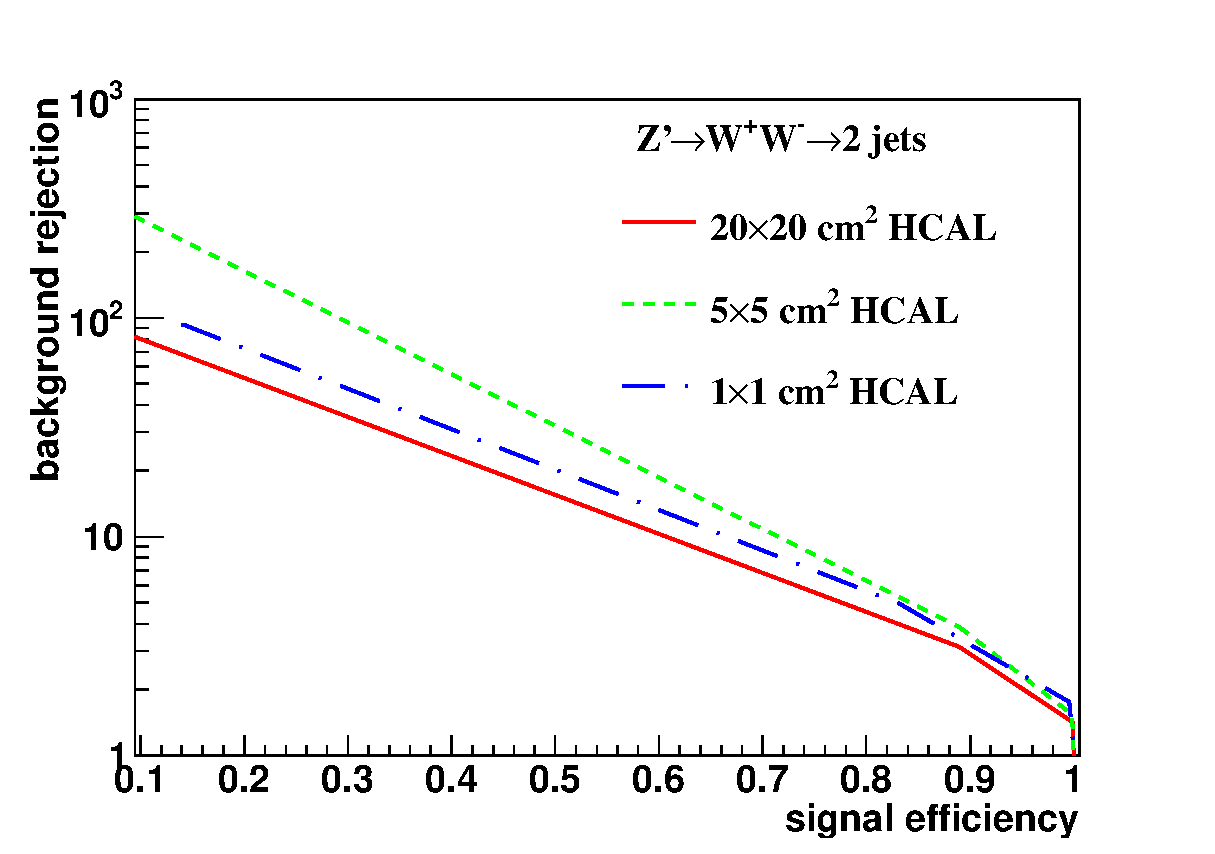
\includegraphics[width=0.43\textwidth]{ROC_Tau_C/Rawhit_05GeV_c2b1_20tev_eff_1_New2_after_cut_25bins_no_UOF_new_75pa.eps}
   }
   \subfigure[Z'(40 TeV)] {
   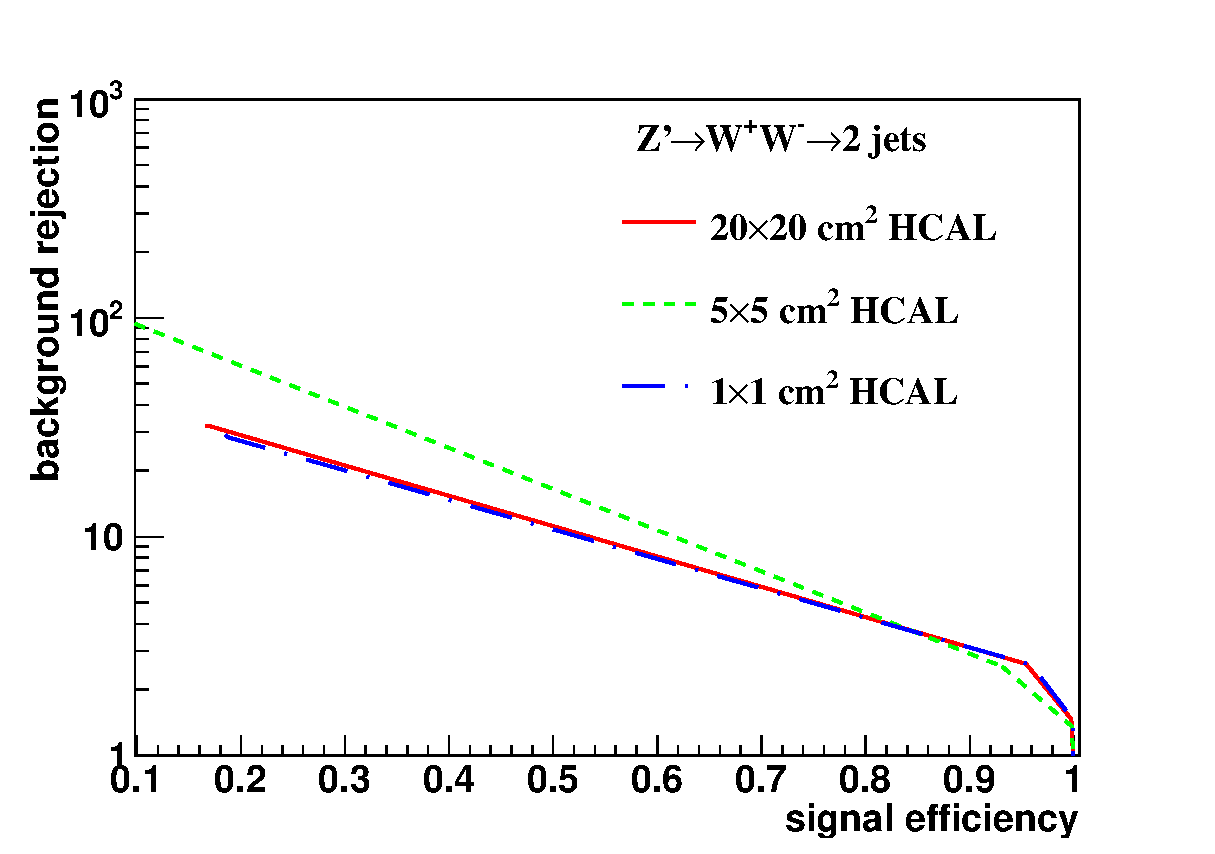
\includegraphics[width=0.43\textwidth]{ROC_Tau_C/Rawhit_05GeV_c2b1_40tev_eff_1_New2_after_cut_25bins_no_UOF_new_75pa.eps}
   }
\end{center}
\caption{Signal efficiency versus background rejection rate using c2b1.The energies of collision at (a)5, (b)10, (c)20, (d)40TeV are shown here. In each picture, the three ROC curves correspond to different detector sizes.}
\label{fig:Rawhit_05GeV_c2b1_ROC}
\end{figure}



%25bins
\begin{figure}
\begin{center}
   \subfigure[20$\times$20($cm^2$)] {
   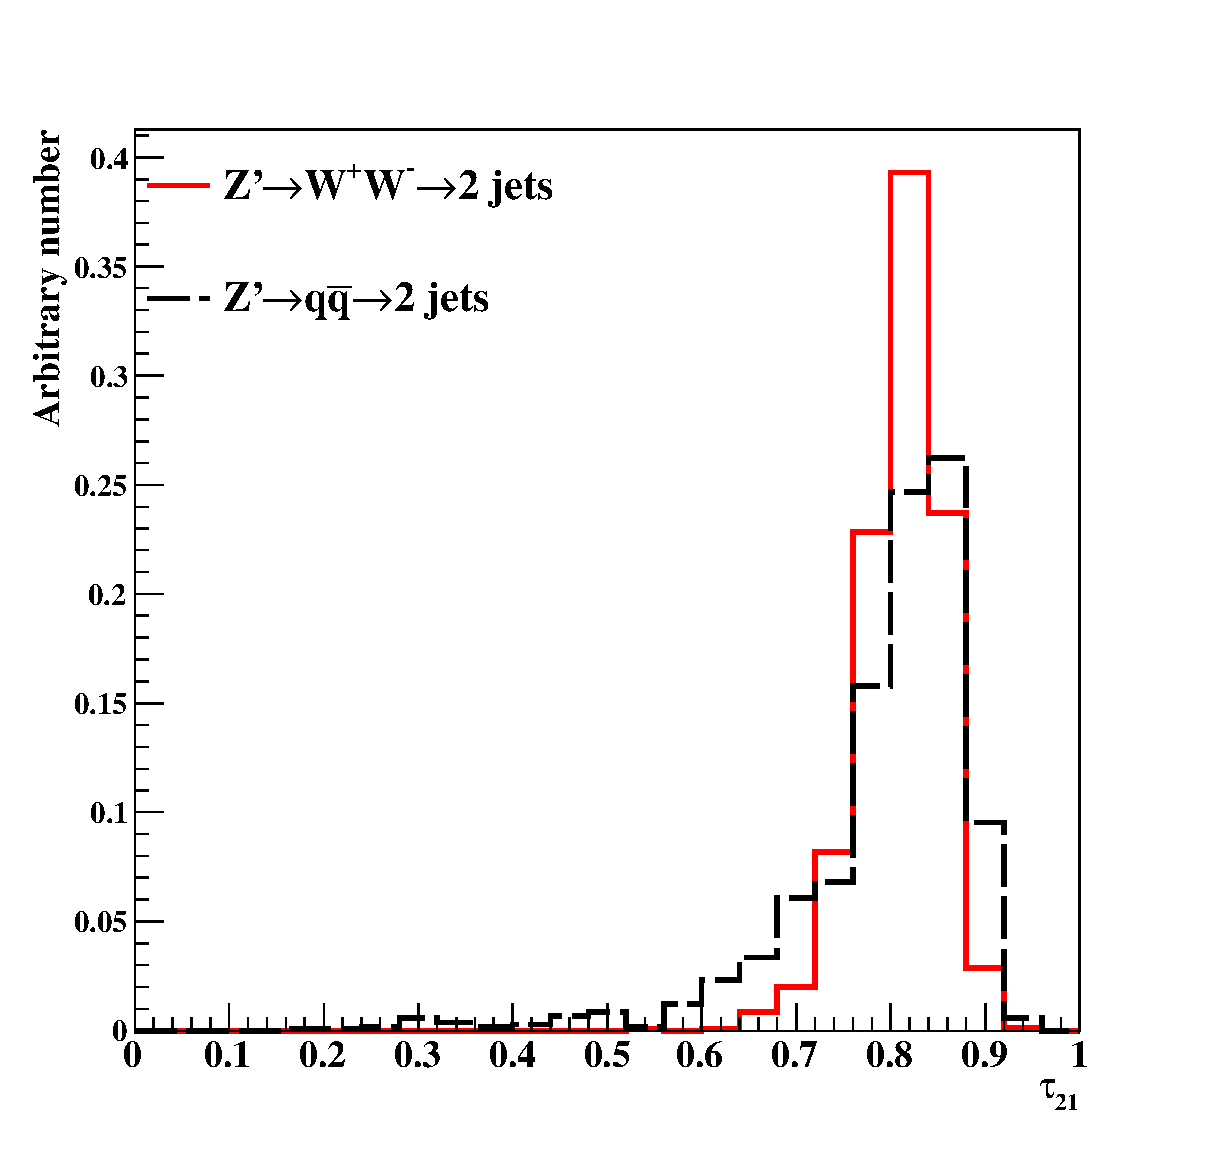
\includegraphics[width=0.3\textwidth]{h_Tau_C/Dis_Rawhit_05GeV_010_tau21_20tev_04_after_cut_Man_25_no_UOF_new_75pa_for_paper.eps}
   }
   \subfigure[5$\times$5($cm^2$)] {
   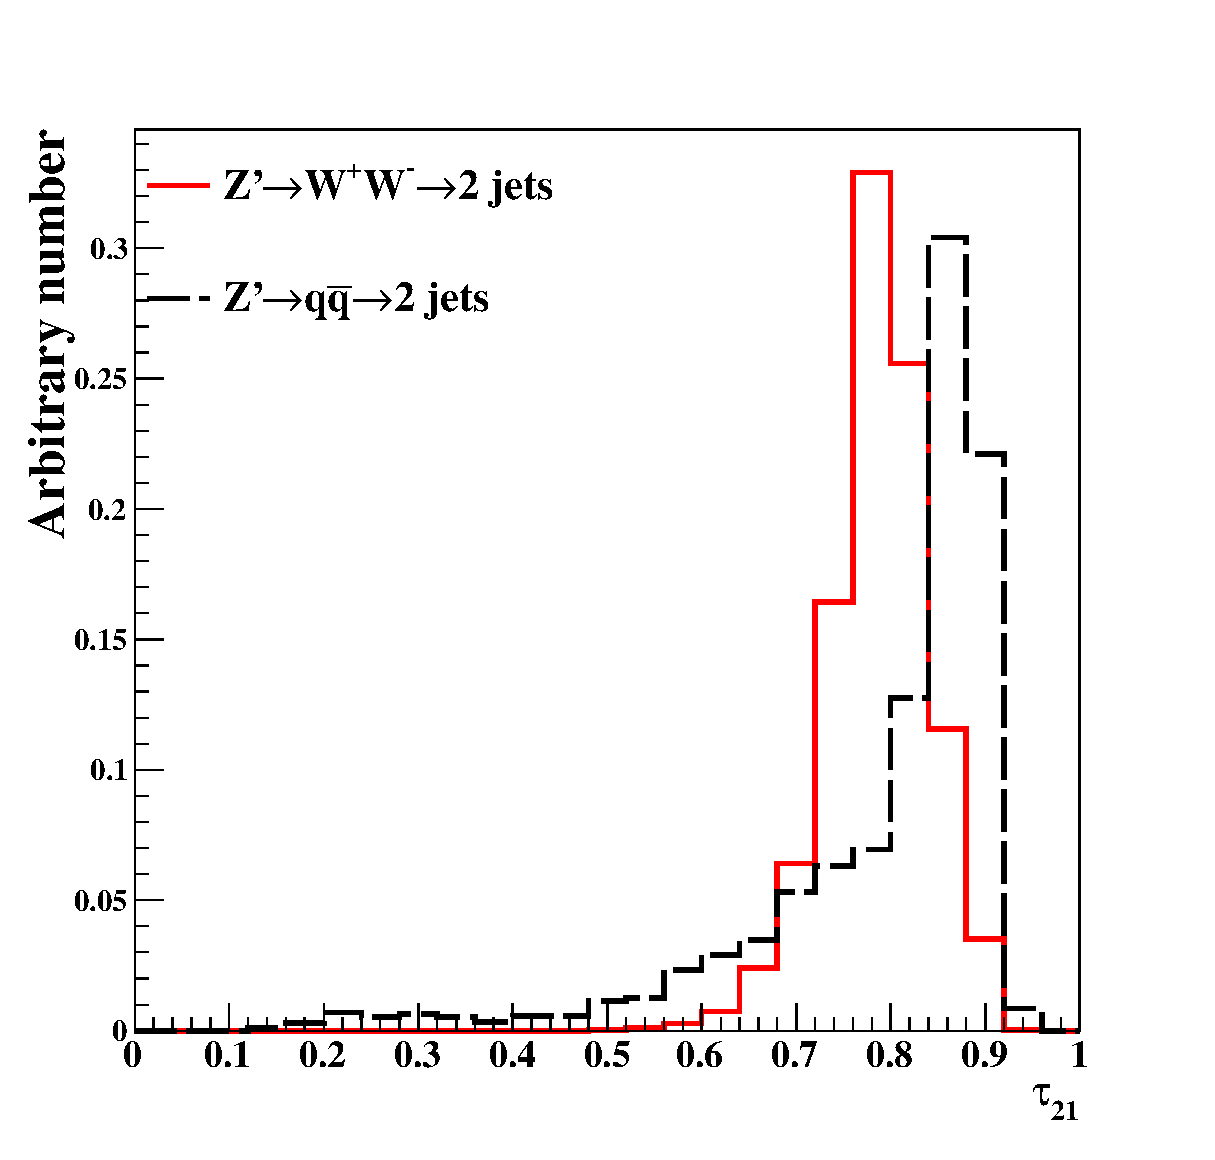
\includegraphics[width=0.3\textwidth]{h_Tau_C/Dis_Rawhit_05GeV_009_tau21_20tev_04_after_cut_Man_25_no_UOF_new_75pa_for_paper.eps}
   }
   \subfigure[1$\times$1($cm^2$)] {
   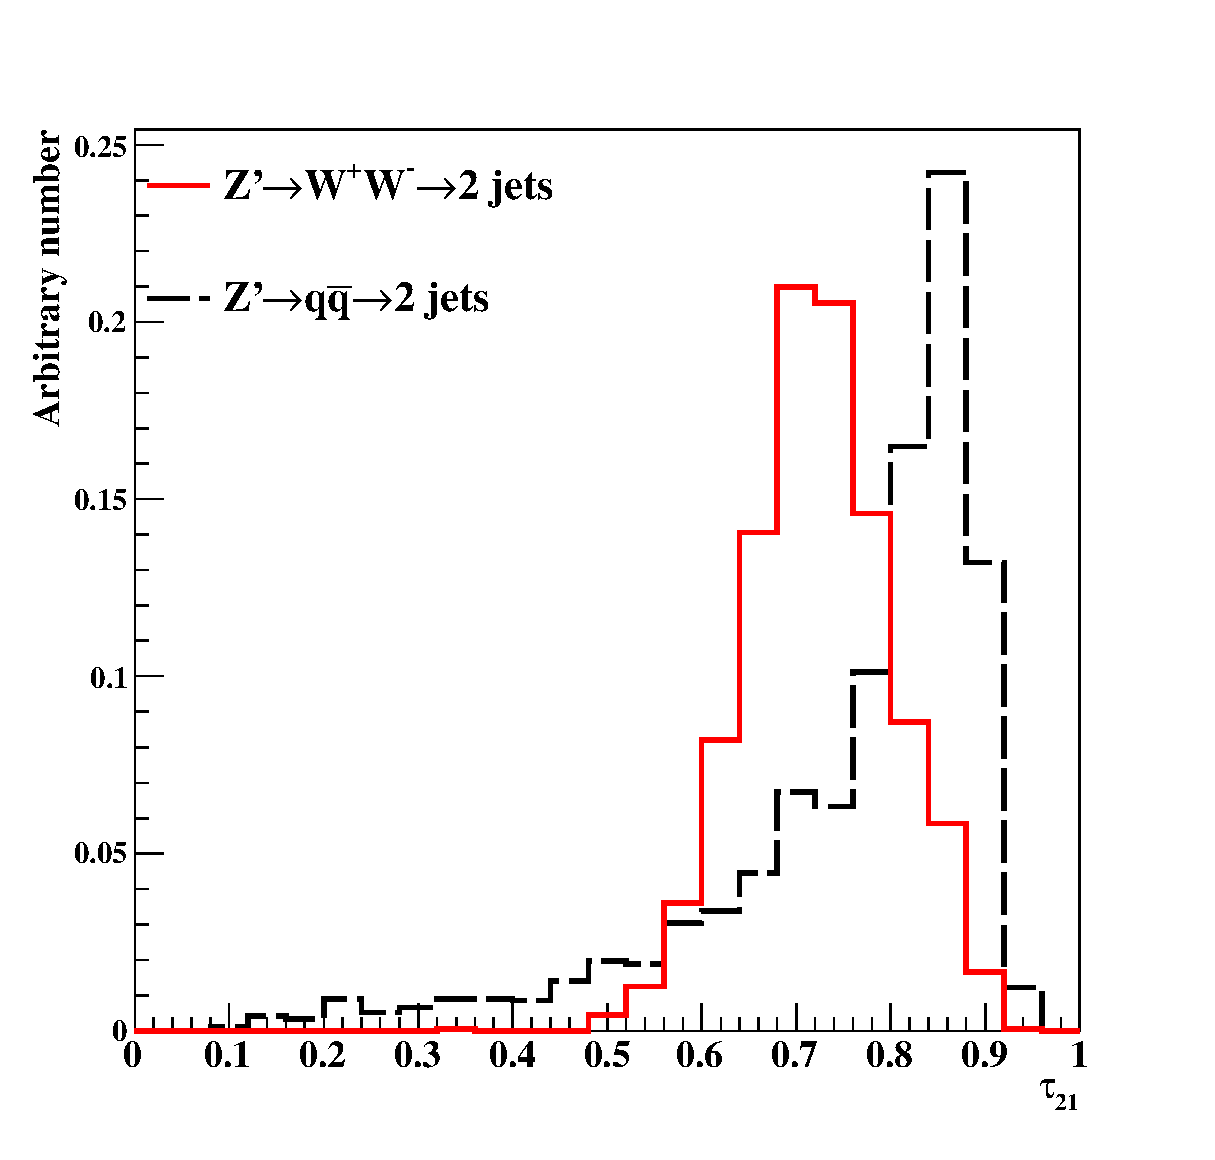
\includegraphics[width=0.3\textwidth]{h_Tau_C/Dis_Rawhit_05GeV_012_tau21_20tev_04_after_cut_Man_25_no_UOF_new_75pa_for_paper.eps}
   }
\end{center}
\caption{Distributions of Mann-Whitney value U in 20 TeV energy collision for $\tau_{21}$  in different detector sizes. Cell Size in 20$\times$20, 5$\times$5, and 1$\times$1(cm$\times$cm) are shown here.}
\label{fig:Rawhit_05GeV_tau21_Dis}
\end{figure}

\begin{figure}
\begin{center}
   \subfigure[Z'(5 TeV)] {
   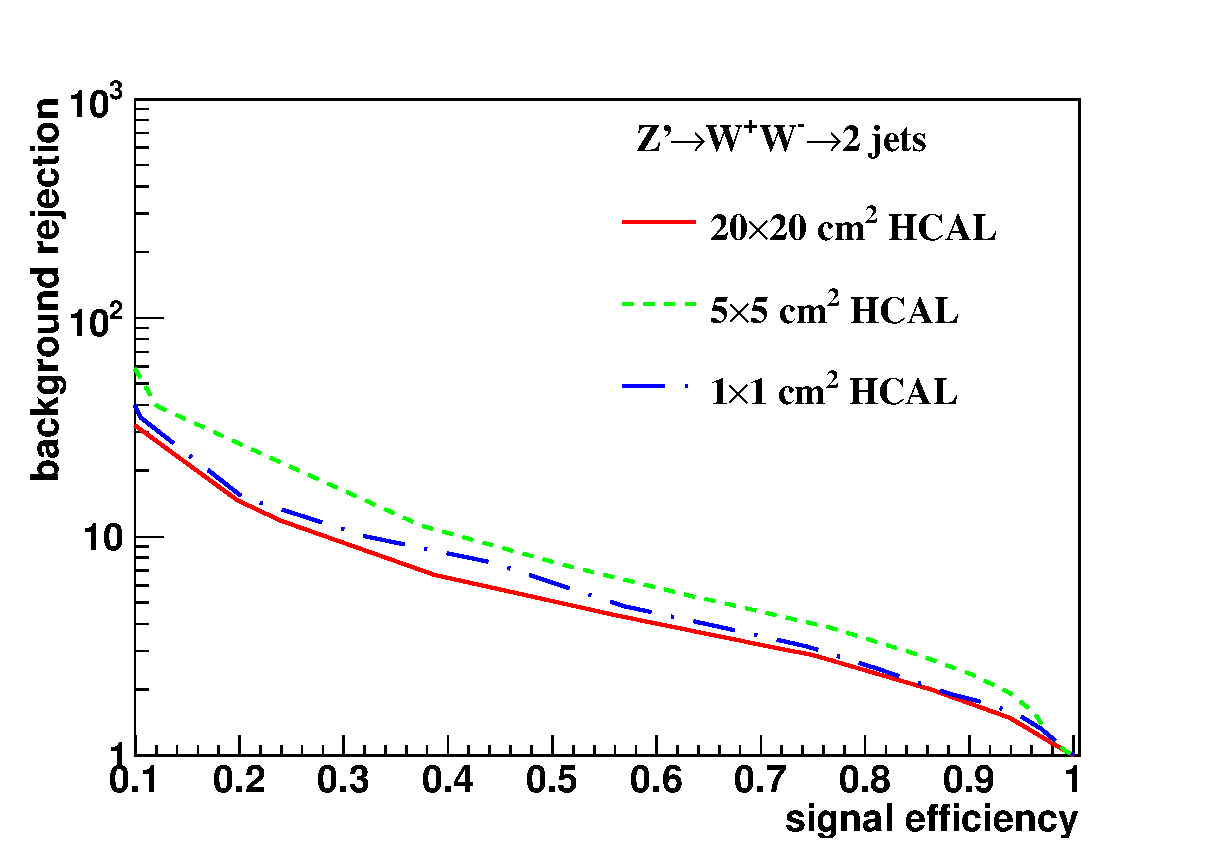
\includegraphics[width=0.43\textwidth]{ROC_Tau_C/Rawhit_05GeV_tau21_5tev_eff_1_New2_after_cut_25bins_no_UOF_new_75pa.eps}\hfill
   }
   \subfigure[Z'(10 TeV)] {
   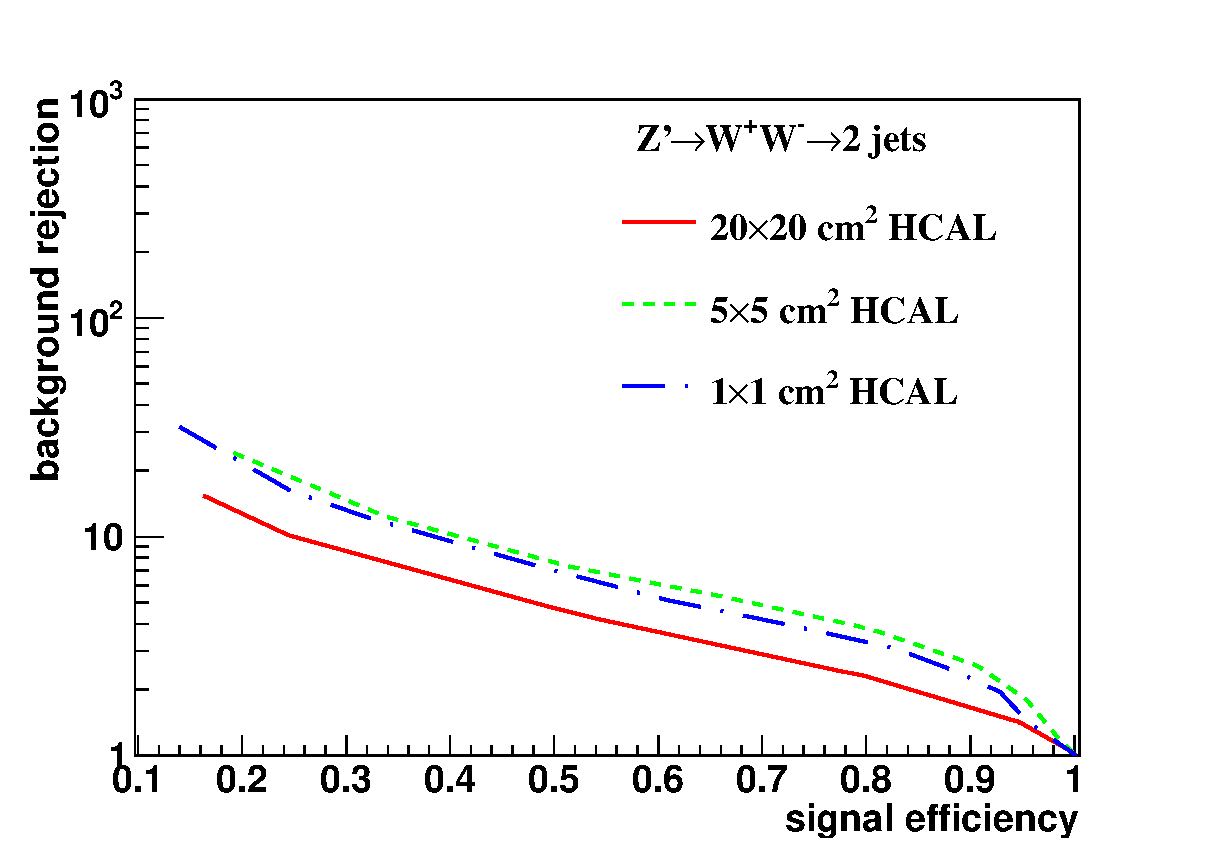
\includegraphics[width=0.43\textwidth]{ROC_Tau_C/Rawhit_05GeV_tau21_10tev_eff_1_New2_after_cut_25bins_no_UOF_new_75pa.eps}
   }
   \subfigure[Z'(20 TeV)] {
   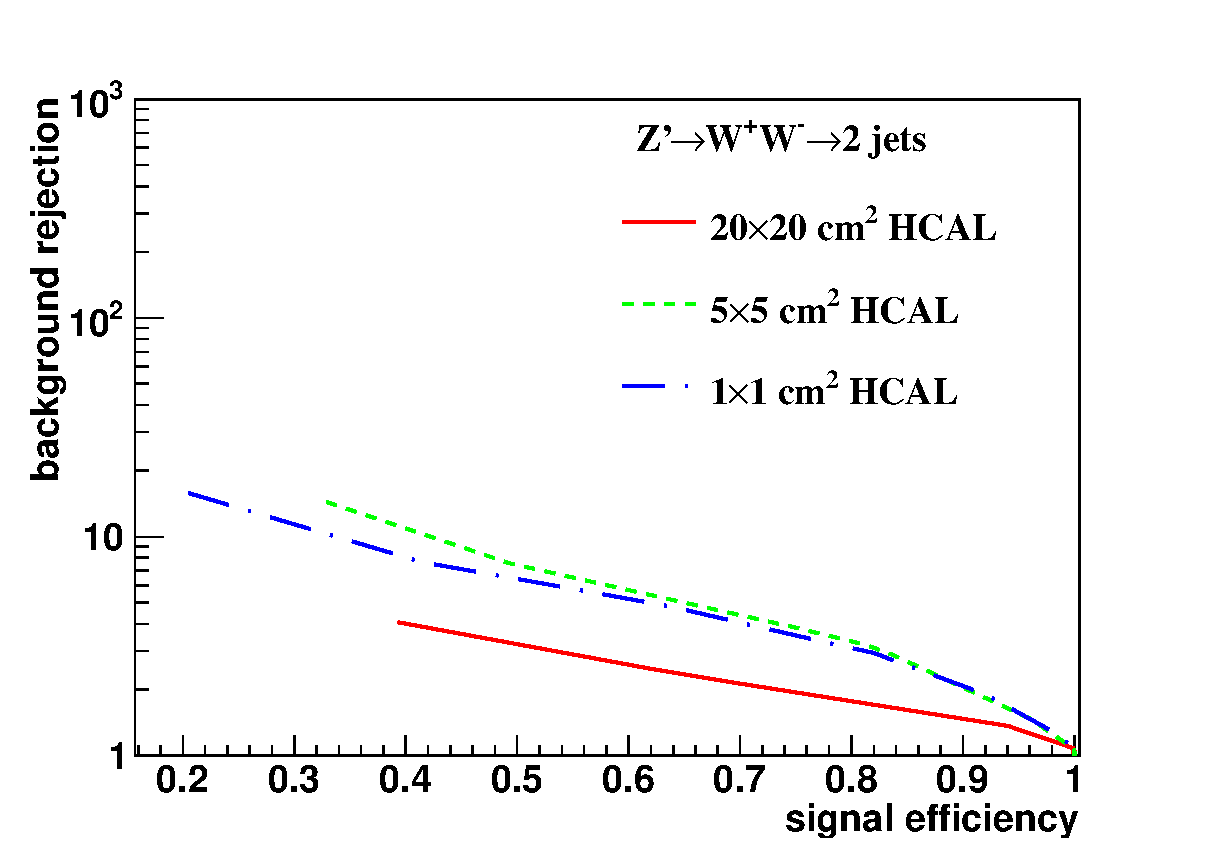
\includegraphics[width=0.43\textwidth]{ROC_Tau_C/Rawhit_05GeV_tau21_20tev_eff_1_New2_after_cut_25bins_no_UOF_new_75pa.eps}
   }
   \subfigure[Z'(40 TeV)] {
   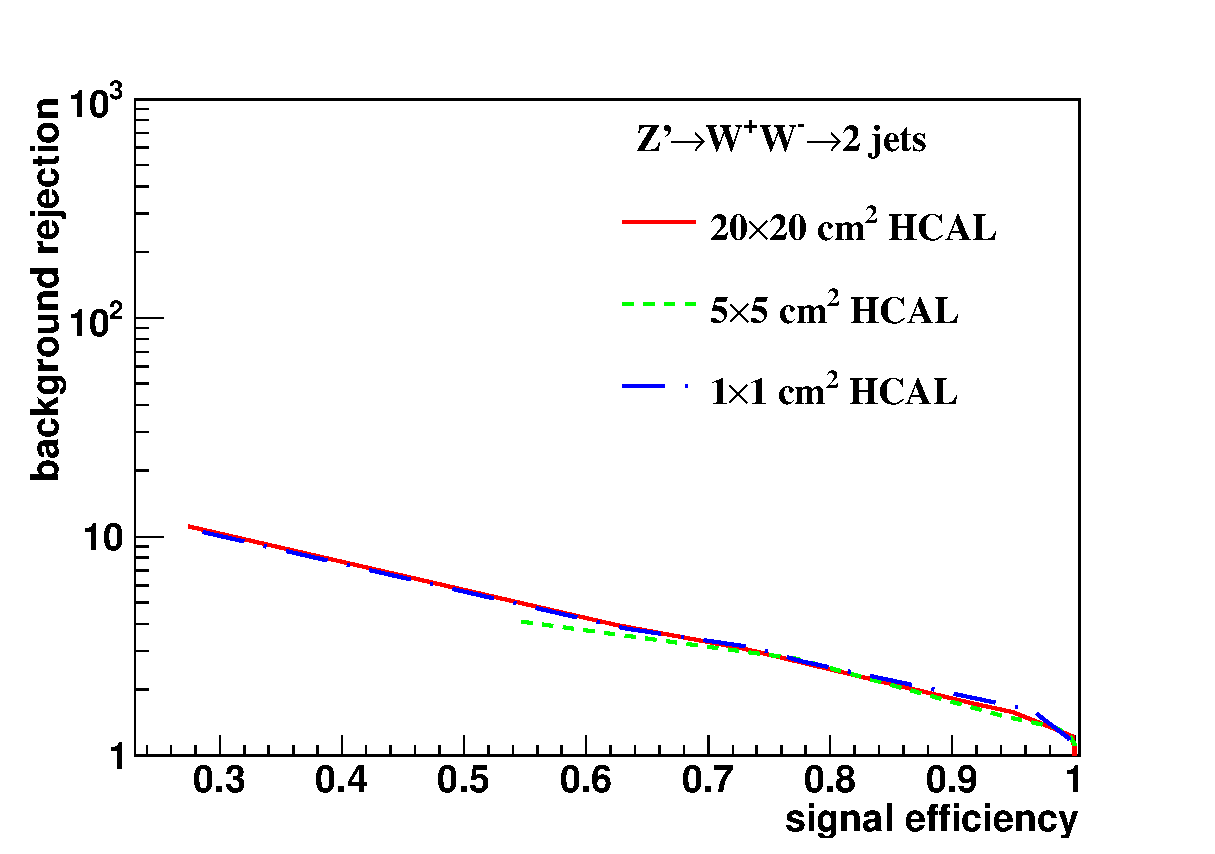
\includegraphics[width=0.43\textwidth]{ROC_Tau_C/Rawhit_05GeV_tau21_40tev_eff_1_New2_after_cut_25bins_no_UOF_new_75pa.eps}
   }
\end{center}
\caption{Signal efficiency versus background rejection rate using $\tau_{21}$.The energies of collision at (a)5, (b)10, (c)20, (d)40TeV are shown here. In each picture, the three ROC curves correspond to different detector sizes.}
\label{fig:Rawhit_05GeV_tau21_ROC}
\end{figure}




%25bins
\begin{figure}
\begin{center}
   \subfigure[20$\times$20($cm^2$)] {
   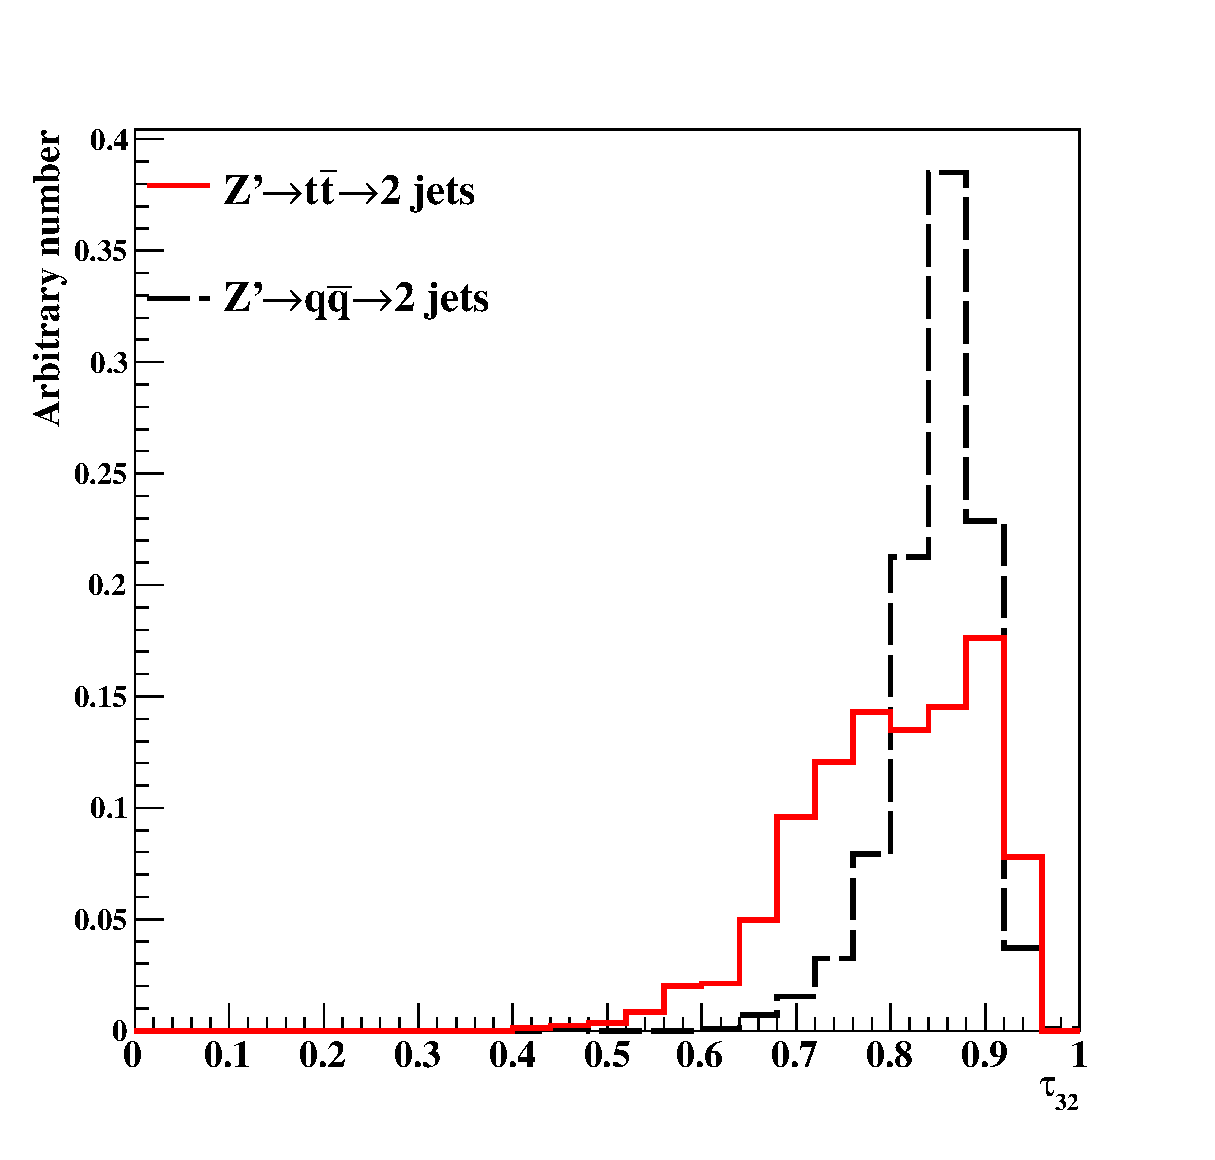
\includegraphics[width=0.3\textwidth]{h_Tau_C/Dis_Rawhit_05GeV_010_tau32_20tev_04_after_cut_Man_25_no_UOF_new_75pa_for_paper.eps}
   }
   \subfigure[5$\times$5($cm^2$)] {
   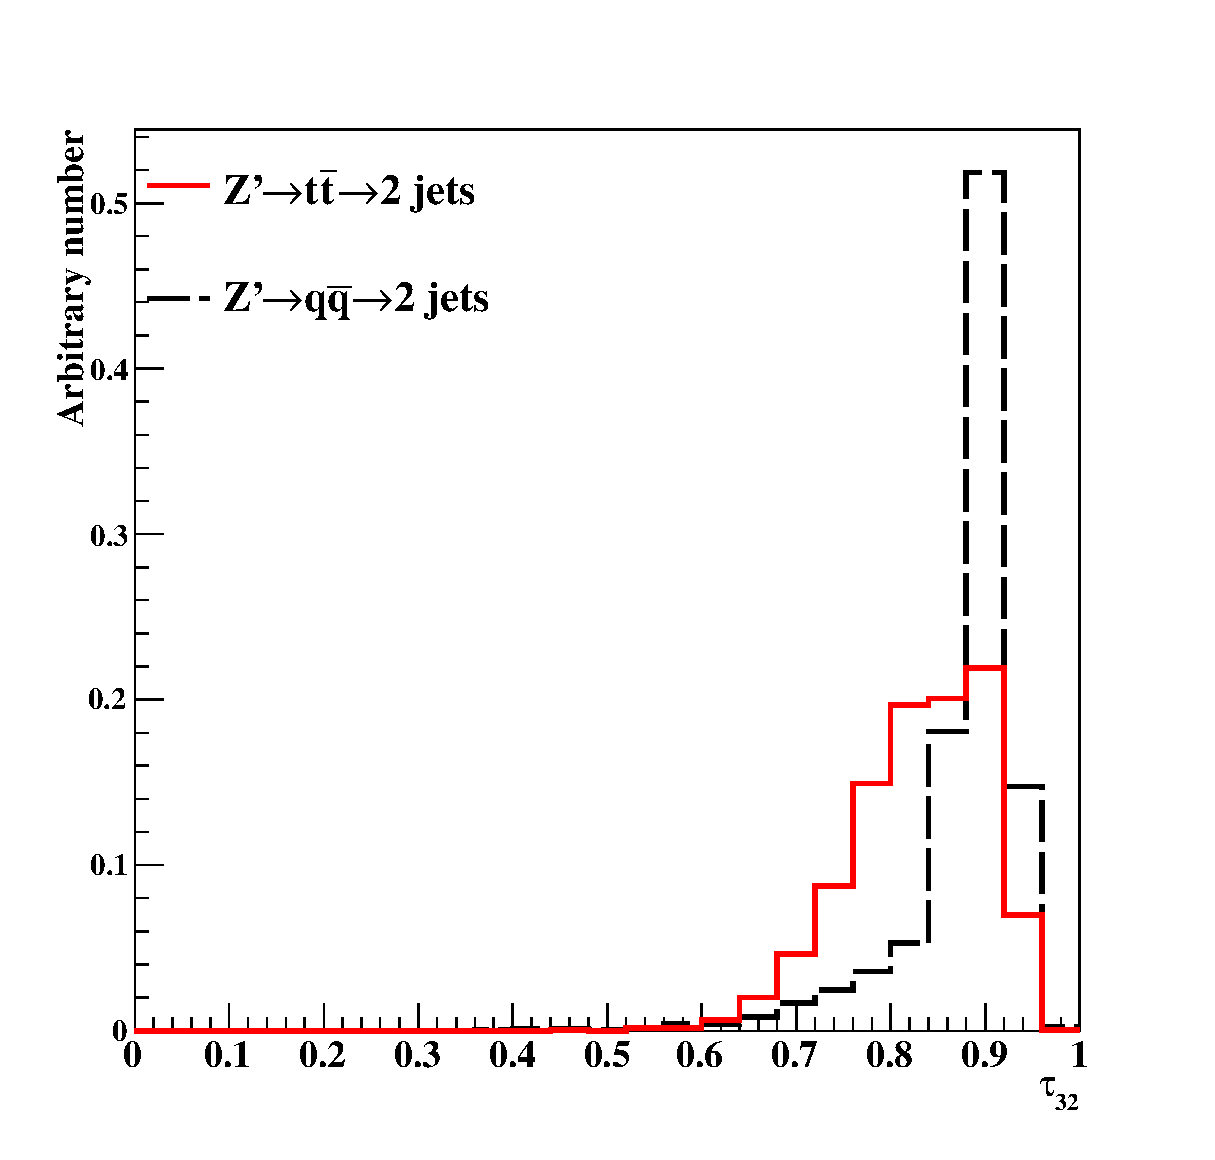
\includegraphics[width=0.3\textwidth]{h_Tau_C/Dis_Rawhit_05GeV_009_tau32_20tev_04_after_cut_Man_25_no_UOF_new_75pa_for_paper.eps}
   }
   \subfigure[1$\times$1($cm^2$)] {
   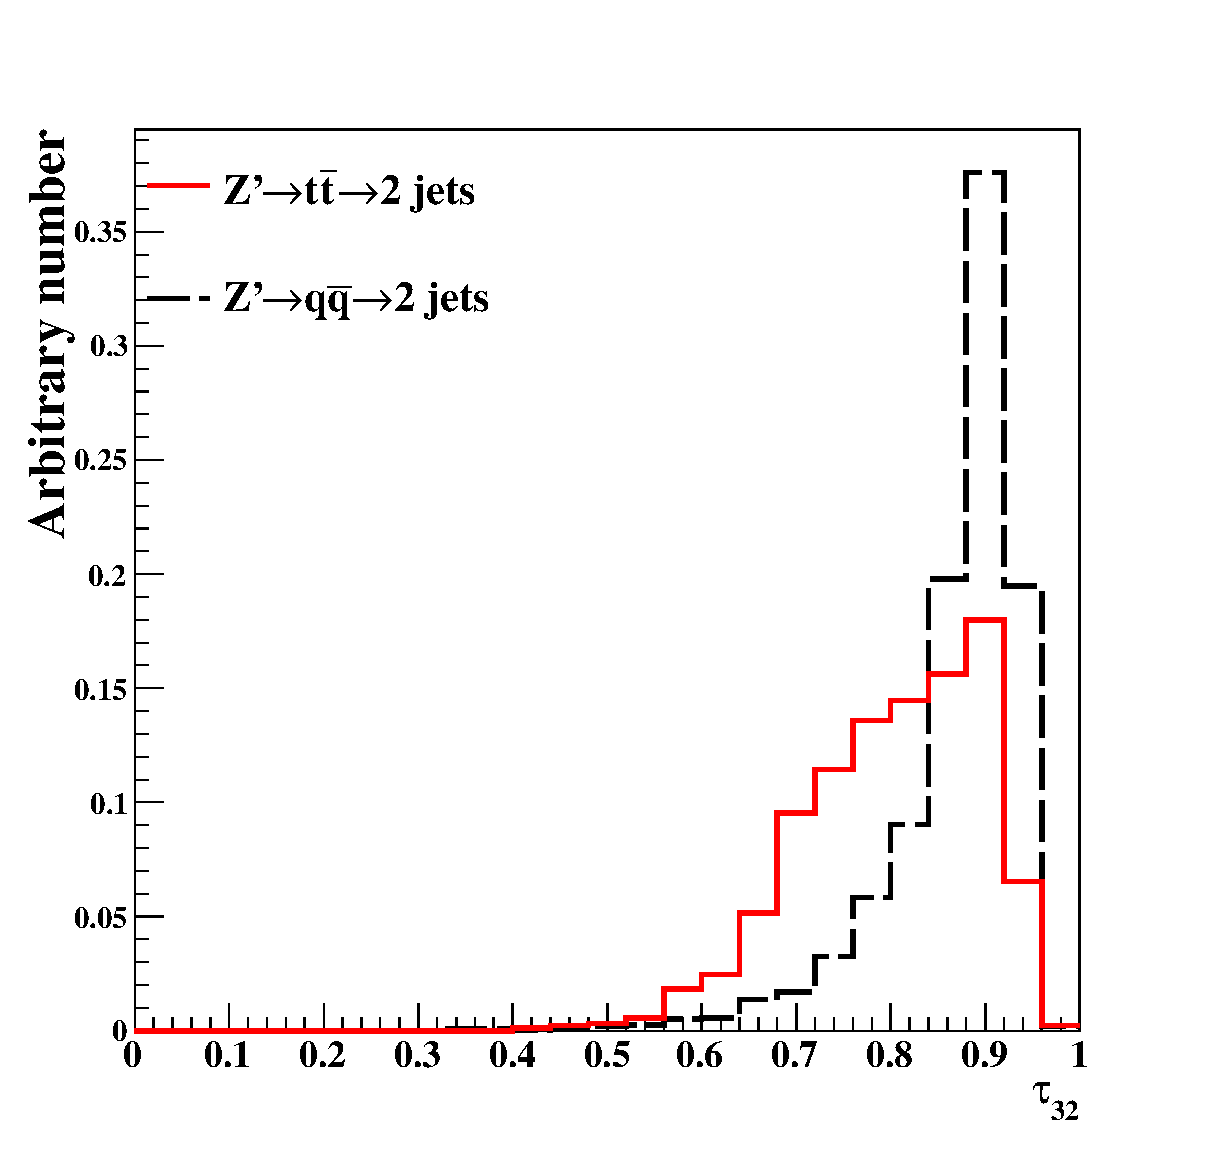
\includegraphics[width=0.3\textwidth]{h_Tau_C/Dis_Rawhit_05GeV_012_tau32_20tev_04_after_cut_Man_25_no_UOF_new_75pa_for_paper.eps}
   }
\end{center}
\caption{Distributions of Mann-Whitney value U in 20 TeV energy collision for $\tau_{32}$  in different detector sizes. Cell Size in 20$\times$20, 5$\times$5, and 1$\times$1(cm$\times$cm) are shown here.}
\label{fig:Rawhit_05GeV_tau32_Dis}
\end{figure}

\begin{figure}
\begin{center}
   \subfigure[Z'(5 TeV)] {
   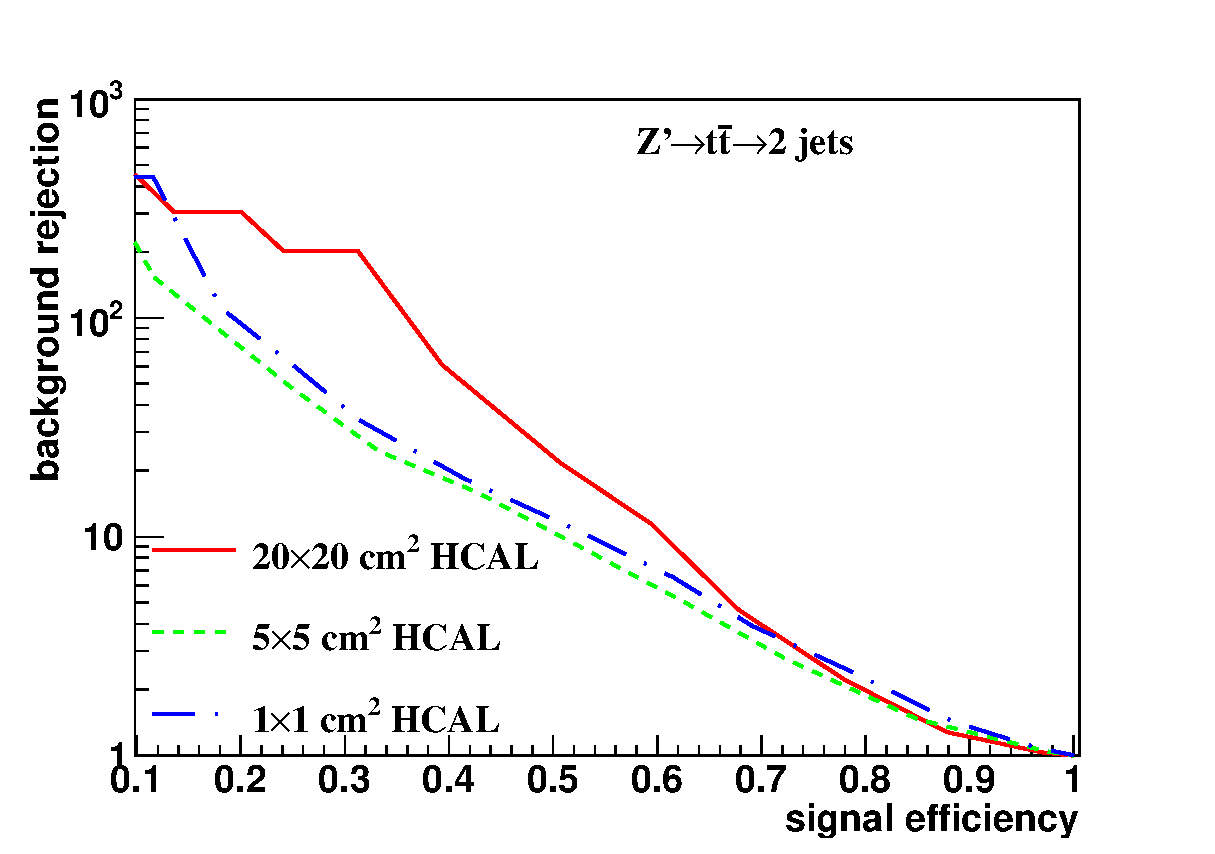
\includegraphics[width=0.43\textwidth]{ROC_Tau_C/Rawhit_05GeV_tau32_5tev_eff_1_New2_after_cut_25bins_no_UOF_new_75pa.eps}\hfill
   }
   \subfigure[Z'(10 TeV)] {
   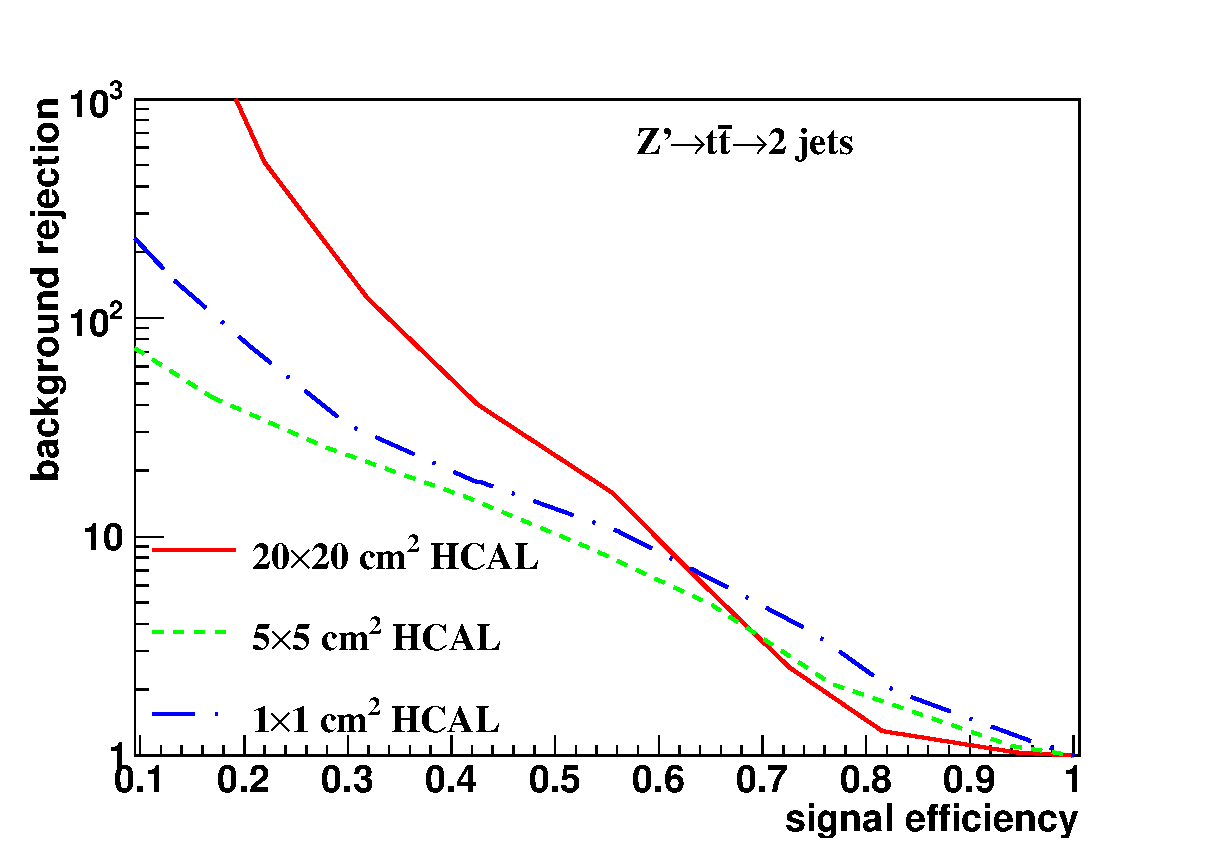
\includegraphics[width=0.43\textwidth]{ROC_Tau_C/Rawhit_05GeV_tau32_10tev_eff_1_New2_after_cut_25bins_no_UOF_new_75pa.eps}
   }
   \subfigure[Z'(20 TeV)] {
   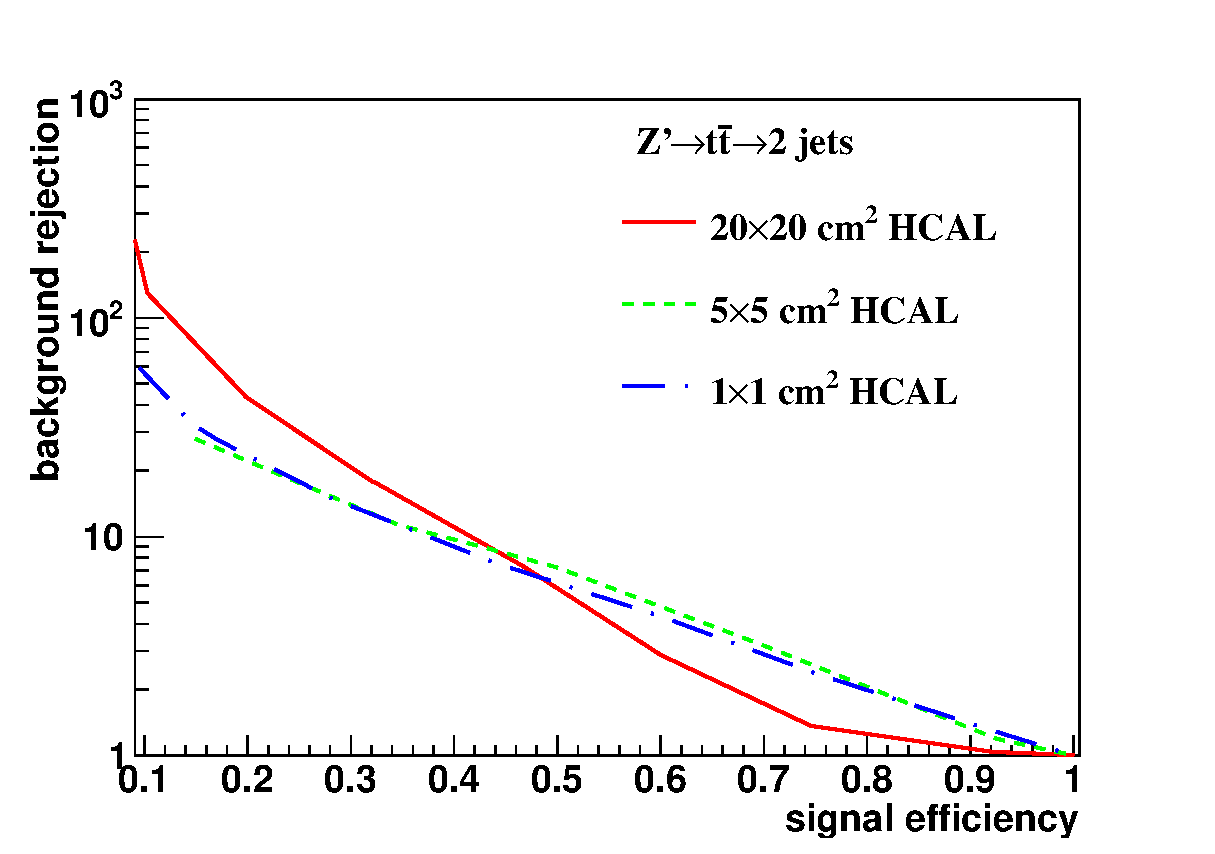
\includegraphics[width=0.43\textwidth]{ROC_Tau_C/Rawhit_05GeV_tau32_20tev_eff_1_New2_after_cut_25bins_no_UOF_new_75pa.eps}
   }
   \subfigure[Z'(40 TeV)] {
   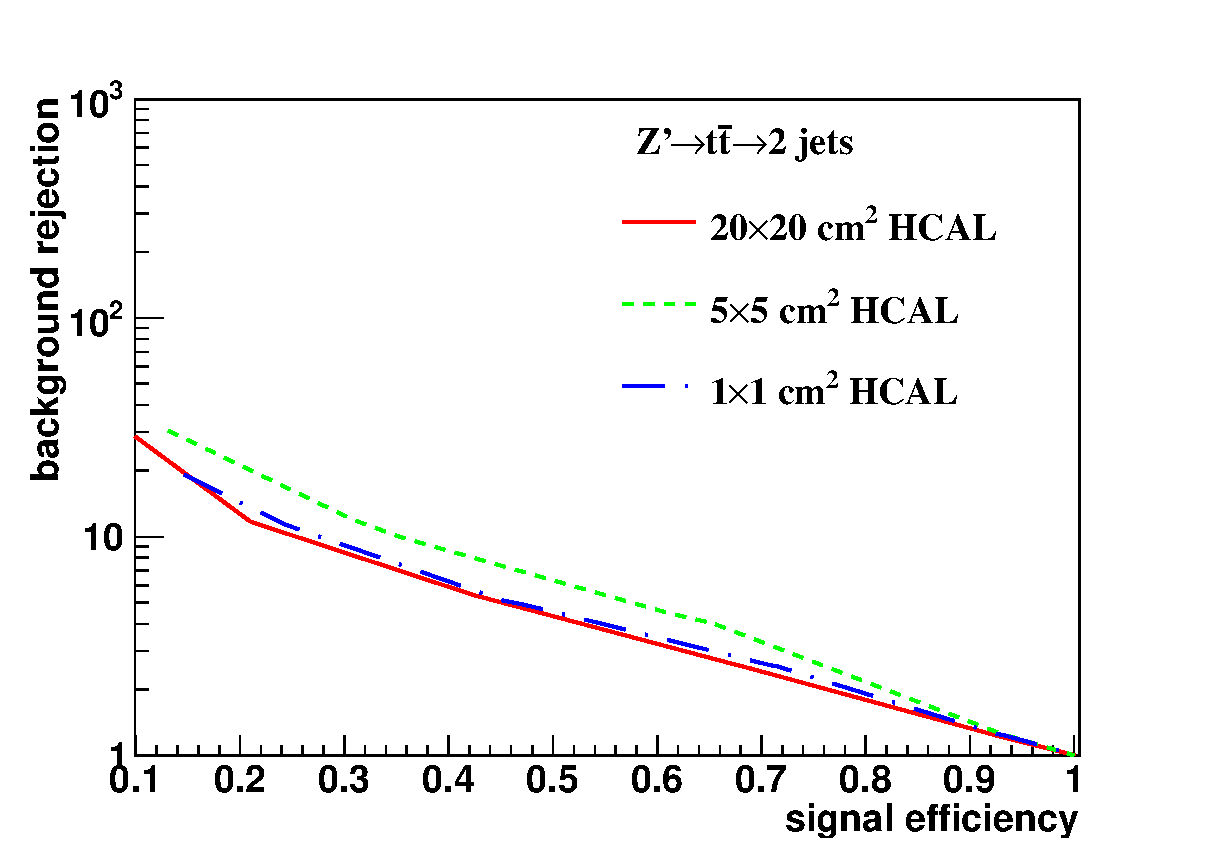
\includegraphics[width=0.43\textwidth]{ROC_Tau_C/Rawhit_05GeV_tau32_40tev_eff_1_New2_after_cut_25bins_no_UOF_new_75pa.eps}
   }
\end{center}
\caption{Signal efficiency versus background rejection rate using $\tau_{32}$.The energies of collision at (a)5, (b)10, (c)20, (d)40TeV are shown here. In each picture, the three ROC curves correspond to different detector sizes.}
\label{fig:Rawhit_05GeV_tau32_ROC}
\end{figure}

%25bins
\begin{figure}
\begin{center}
   \subfigure[$\tau_{21}$] {
   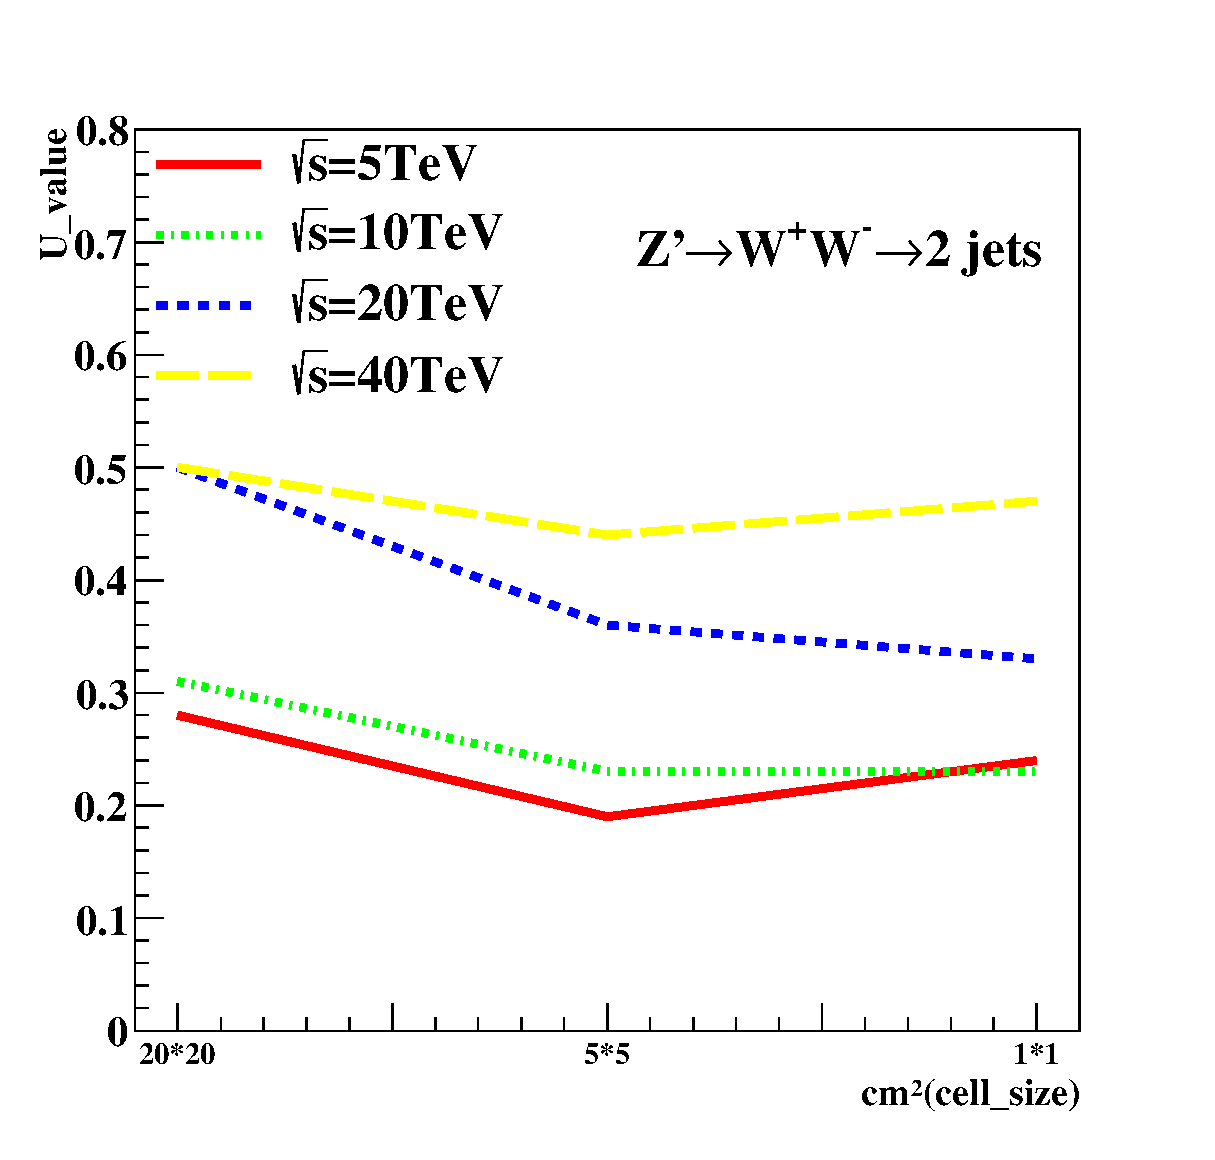
\includegraphics[width=0.3\textwidth]{Mann_Sum/raw_05_tau21_summary_U_after_cut_25bins_no_UOF_new_75pa.eps}\hfill
   }
   \subfigure[$\tau_{32}$ ] {
   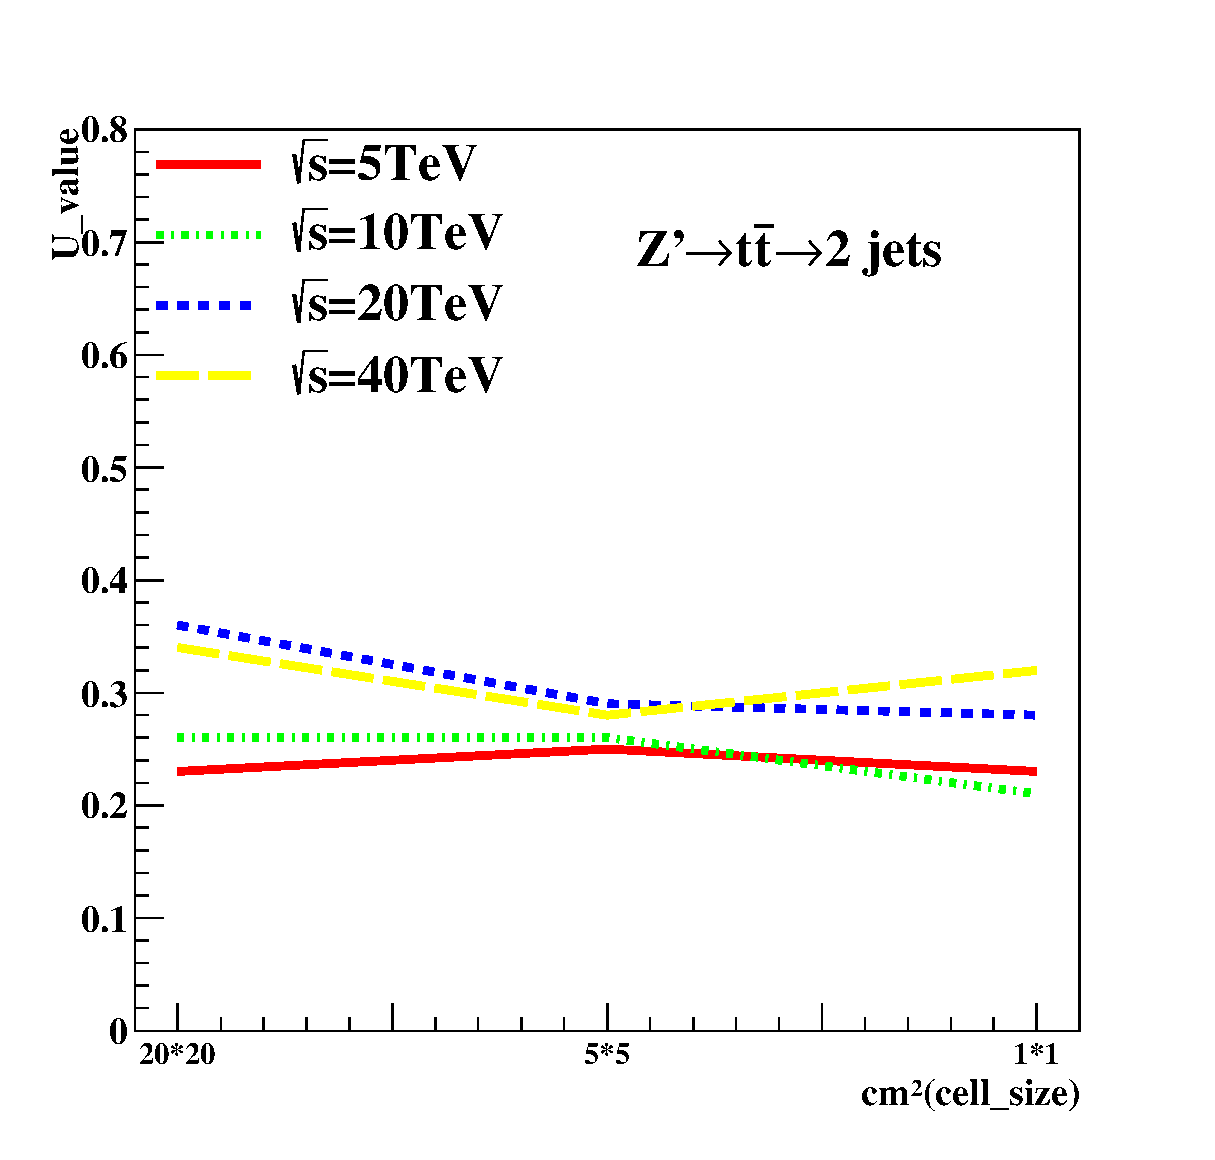
\includegraphics[width=0.3\textwidth]{Mann_Sum/raw_05_tau32_summary_U_after_cut_25bins_no_UOF_new_75pa.eps}
   }
   \subfigure[$c_2^{(1)}$] {
   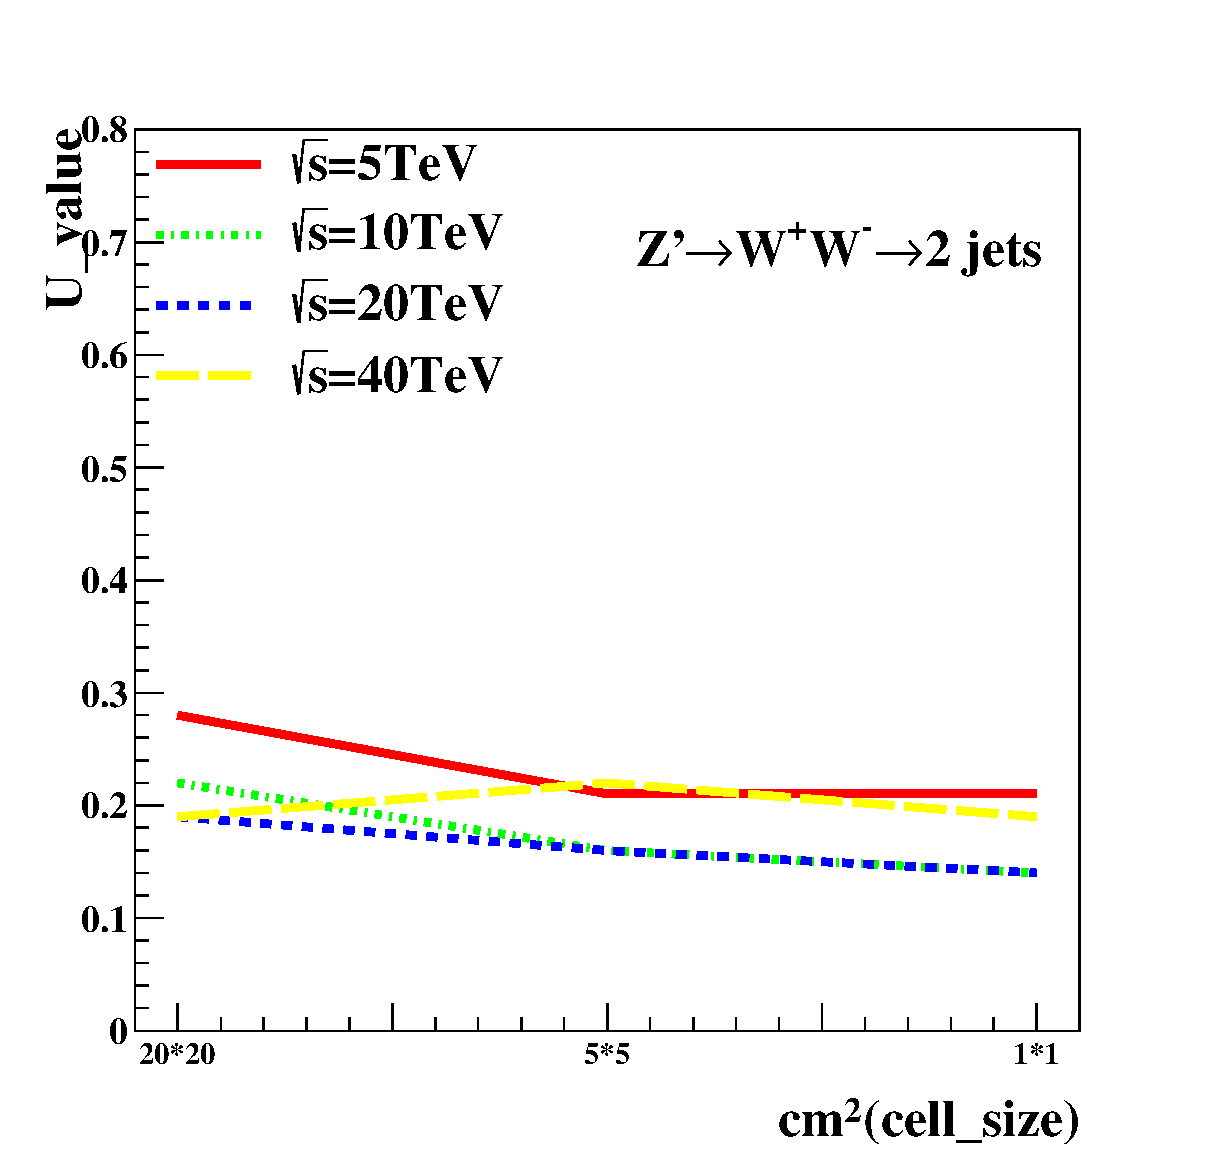
\includegraphics[width=0.3\textwidth]{Mann_Sum/raw_05_c2b1_summary_U_after_cut_25bins_no_UOF_new_75pa.eps}
   }
\end{center}
\caption{The Mann-Whitney U values for $\tau_{21}$,$\tau_{32}$ and $c_2^{(1)}$ reconstructed from calorimeter hit at 05GeV cut with different collision energies correspond to different detector sizes in rawhit cut with 05GeV. The energies of collision at 5, 10, 20, 40, 20, 40TeV are shown in each figure.}
\label{fig:Rawhit_05GeV_total_Mann}
\end{figure}



